% 1977 年湖南株洲卷参考题 3：抛物线拱窗，坐标系原点在抛物线顶点 O，拱脚 A(60,-30)，
% 边高 150、顶点高 180、窗宽 120（单位 cm，图按 1:10 缩绘；按源卷第 10 页布局）
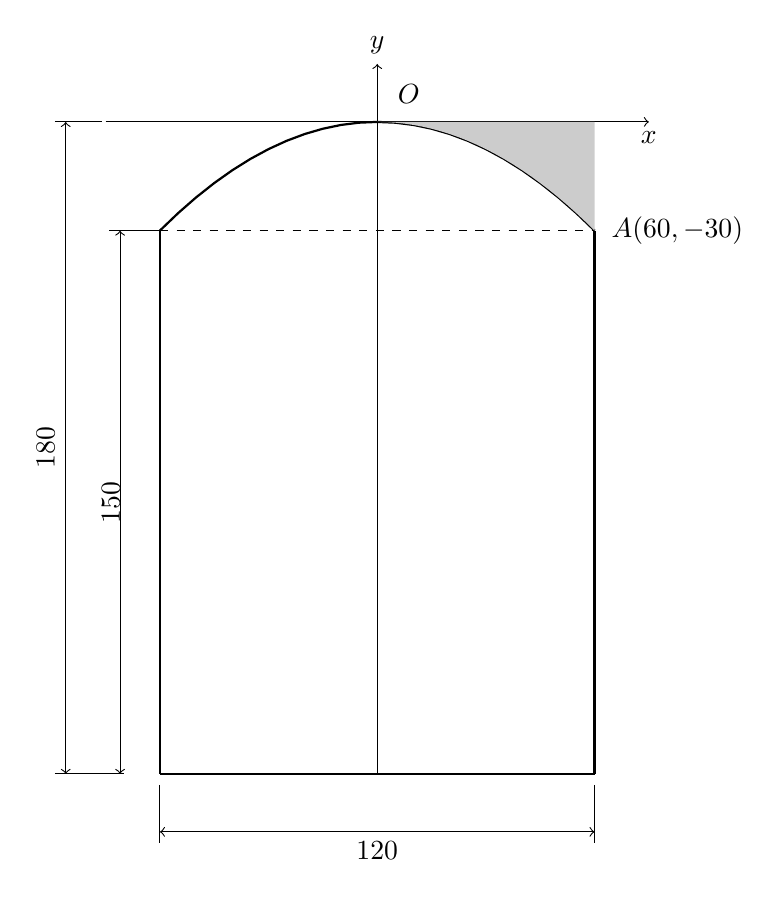
\begin{tikzpicture}[scale=0.46]
  \draw[->] (-7.5,0)--(7.5,0) node[below] {$x$};
  \draw[->] (0,-18)--(0,1.6) node[above] {$y$};
  \draw[thick] plot[domain=-6:6] (\x,{-\x*\x/12});
  \draw[thick] (-6,-3)--(-6,-18);
  \draw[thick] (6,-3)--(6,-18);
  \draw[thick] (-6,-18)--(6,-18);
  \draw[dashed] (-6,-3)--(6,-3);
  \fill[black!20] (0,0) -- plot[domain=0:6] (\x,{-\x*\x/12}) -- (6,0) -- cycle;
  \draw[<->] (-8.6,0)--(-8.6,-18);
  \draw (-8.9,0)--(-7.6,0);
  \draw (-8.9,-18)--(-7.0,-18);
  \node[rotate=90] at (-9.15,-9) {$180$};
  \draw[<->] (-7.1,-3)--(-7.1,-18);
  \draw (-7.4,-3)--(-6,-3);
  \node[rotate=90] at (-7.35,-10.5) {$150$};
  \draw (-6,-18.3)--(-6,-19.9);
  \draw (6,-18.3)--(6,-19.9);
  \draw[<->] (-6,-19.6)--(6,-19.6);
  \node[below] at (0,-19.6) {$120$};
  \node[above right] at (0.3,0.25) {$O$};
  \node[right] at (6.2,-3) {$A(60,-30)$};
\end{tikzpicture}
